\chapter{Lecture 8: Random variables, probability mass functions, and cumulative distribution functions} \label{lec8}
A \textbf{random variable} is a variable that takes a numerical value for each possible outcome of a statistical experiment. The value that the random variable takes will depend on the outcome of the experiment, which is random; hence the name. We generally use upper case letters from the end of the alphabet (say $X, Y,$ or $Z$) to denote random variables. The following example should give you a better idea of what a random variable is (and what randomness means in this context).

\subsection{Example} \label{example8.1}
Consider again the two dice experiment from example \ref{example2.2.1}. Recall the events
\begin{align*}
A & = \set{\text{The total shown on the two dice is 6}} \\
B & = \set{\text{The total shown on the two dice is 2}}.
\end{align*}
The events, $A$ and $B$, are both collections of \textit{elementary} events (i.e., outcomes). Since every outcome is represented by a pair of numbers, we can always find their sum. This \textit{property} that is shared by all of the outcomes (their sum) can be used to define 9 more similar events; i.e., we can specify a total of 11 events by referring to the sum of the two dice (the sum can be 2,3,4,5,6,7,8,9,10,11, or 12). \\

\noindent This property (the sum) can be represented by a variable, say $X$. We just define $X$ to be a variable that can take values from the set of all possible sums of two dice, i.e., let $X \in \set{2,3,4,5,6,7,8,9,10,11,12}$. That is, $X$ can be any natural number where $2 \leq X \leq 12.$ The value of $X$ is not pre-determined, so we call $X$ a \textbf{random variable.} \label{random variable} \\

\noindent We just said that \textit{the value of $X$ is not predetermined.} However, it is not hard to see that we are more \textit{likely} to roll a $7$ on two dice, than we are to roll a $2$. This is because there are more ways to roll a 7 than there are ways to roll a 2. The outcome of each \textit{individual} roll is completely random and unpredictable; but, upon analysing many rolls, we will see a pattern in which $X = 7$ occurs more often than $X = 2$. It is interesting that the underlying process (outcome of rolling a die) is governed by randomness (hence describable by a random variable), yet we observe a distinct, predictable pattern. Patterns like these give us information about the nature of a phenomenon; for example, if we analyse many rolls and find that 2 appears more often than 7, then we might make a conclusion that the dice are not fair, or that the underlying process is not random, or perhaps that the dice are not numbered from 1 to 6 (or that we have not analysed enough rolls).

\subsection{Random variables are functions} \label{sec8.10}
It might sound strange to hear us refer to a variable as a function, but, in fact, a random variable, say $Z$, \textit{is} a function. The domain of $Z$ is the universal set, $\Omega$, and its codomain is $\R$. In other words, $Z$ maps elements of $\Omega$ to some subset of the real numbers. In the previous example (example \ref{example8.1}), $X$ was a random variable whose input was the values of two dice, and whose output was the sum of the two dice. Hence, for example
\[
X((1,1)) = 1 + 1 = 2, \qquad X((4,5)) = 4 + 5 = 9, \qquad X((6,2)) = 6 + 2 = 8
\]
In this case, the possible outputs of $X$ are the natural numbers between 2 and 12 (which is indeed a subset of the real numbers). \\

\noindent Notice that, since $X$ is a function, we only assign one unique value to each outcome in the domain of $X$. This means that, for some arbitrary outcome, $a$, we cannot have, for example, $X(a) = 2$ \textit{and} $X(a) = 3$. As we will soon see (in section \ref{disjran}), this means that different events specified by a random variable will always be disjoint. \\

\noindent Also, functions by definition always map every element in their domain to somewhere, so random variables assign some output to every element in \textit{their} domain, $\Omega$. This means that the events specified by random variables are exhaustive (they cover the whole sample space). \\

\noindent The fact that the events specified by a random variable are collectively always disjoint and exhaustive is important and will come up (somewhat subtly) many times during this course.

\subsection{Probability measures and random variables} \label{sec8.1}
Recall that probability measures must always take \textit{events} as their inputs; i.e., probability measures are functions which assign probabilities (real numbers) to particular \textit{events} (subsets of $\Omega$). What if we want to use a probability measure, let's call it $p(x)$, to assign a probability to each output of a random variable, say $Z$? Then $p(x)$ will still need to have the $\textit{events}$ themselves as its domain. \\

\noindent Since $Z$ is a random variable, it has events as its domain, but its outputs are not events, they are real numbers. We want $p(x)$ to associate probabilties with the \textit{outputs} of $Z$. The following definition will allow this to happen: \\

\noindent Let $Z$ be a random variable, and let $z$ represent one of the particular values that $Z$ can take. We define \label{symbZ=z}

  	\bigskip
	
	\hfil\fbox{
	\begin{minipage}{0.6\columnwidth}{
	
	\vskip 0.02cm
	\begin{center}
	$\set{Z = z}\;\; \text{is shorthand for} \;\; \set{\omega \in \Omega \mid Z(\omega) = z}$
	\end{center}
	}
	\end{minipage}}
	\bigskip
	\bigskip
	
\noindent So, using $X$ from example \ref{example8.1} we get, for example,
\[
\set{X = 4} \;\; = \;\; \set{\omega \in \Omega \mid X(\omega) = 4} = \set{(2,2),(3,1),(1,3)}.
\]
\noindent In other words, we define $\set{X = 4}$ to be shorthand for the set of outcomes which are mapped to the number $4$ by $X$, i.e., the \textit{event} which is mapped to $4$ by $X$. For convenience, we sometimes write ``$\set{Z = z}$'' as simply ``$Z = z$.'' \\

\noindent Now we can ask, for example,
\[
\text{What is} \;\; P\brac{X = 4}?
\]
We read this as, ``what is the probability that $X = 4$?'' Using our definition of $X = 4$, we can intepret this as, ``what is the probability of the event that the sum of the two dice is 4?'' In other words, we are asking, ``what is the probability of the event, $\set{(2,2),(3,1),(1,3)}$?'' The answer is
\[
P\brac{X = 4} \;\; = \;\; p(\set{(2,2),(3,1),(1,3)}) = \frac{3}{36} = \frac{1}{12}.
\]
Similarly, we can now find the probability that $X$ will fall within a particular interval. For example,
\[
\text{What is} \;\; P(2 \leq X \leq 4)?
\]
We interpret the expression $\set{2 \leq X \leq 4}$ as shorthand for $\set{\omega \in \Omega \mid 2 \leq X(\omega) \leq 4}.$ In other words,
\[
\set{2 \leq X \leq 4} \;\; = \;\; \set{X = 2} \cup \set{X = 3} \cup \set{X = 4}.
\]
We are asking, ``what is the probability that $X$ is between 2 and 4?'' \\

\noindent How do we find $P(\set{X = 2} \cup \set{X = 3} \cup \set{X = 4})?$ We could use the addition law if we knew that the sets $\set{X = 2}, \set{X = 3}$ and $\set{X = 4}$ are disjoint. Indeed they are disjoint; we already mentioned in section \ref{sec8.10} that the events that are specified by a random variable are always disjoint. We will prove this in the next section.

\subsection{Disjoint events and random variables} \label{disjran}
In general, if we have two random variables, $X$ and $Y$, the events that they specify might not be disjoint. That is, for example, $\set{X = 1}$ might not be disjoint from the set $\set{Y = 2}$. However, if we restrict ourselves to one random variable, $X$, with $k_1$ and $k_2$ being two possible outputs of $X$, then
\[
\set{X = k_1} \qquad \text{is disjoint from} \qquad \set{X = k_2}
\] 
so long as $k_1 \neq k_2$. The following arrow diagram will help us understand this fact, the diagram is a visualisation of a random variable as a function:
\begin{center}
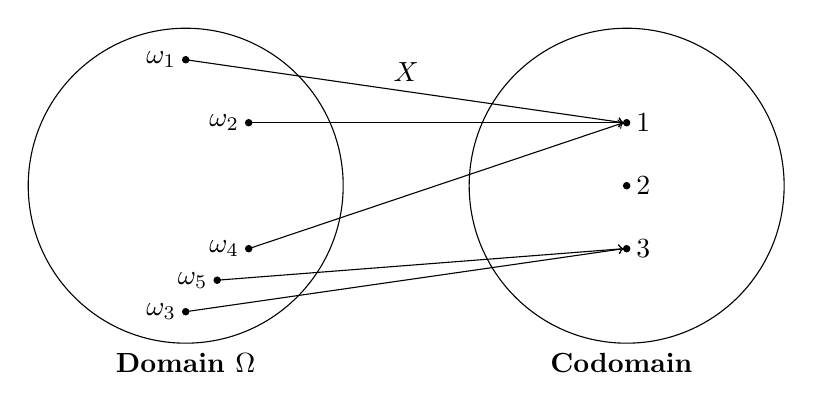
\begin{tikzpicture} [scale = 0.8]
	\draw (0,0) circle (2.5cm) node [below = 2cm] {\textbf{Domain $\Omega$}};
	\draw (7,0) circle (2.5cm) node [below = 2cm] {\textbf{Codomain $\R$}};
	
	\draw [fill = black] (0,2) circle (0.05cm) node [left] {$\omega_1$};
	\draw [fill = black] (1,1) circle (0.05cm) node [left] {$\omega_2$};
	%\draw [fill = black] (0.5,1.5) circle (0.05cm) node [left] {$\omega_3$};
	\draw [->] (1,1) -- (7-0.05,1);
	\draw [->] (0,2) -- (7-0.05,1);
	%\draw [->] (0.5,1.5) -- (7-0.05,1);
	\draw [->] (1,-1) -- (7-0.05,1);
	
	\draw [fill = black] (0,-2) circle (0.05cm) node [left] {$\omega_3$};
	\draw [fill = black] (1,-1) circle (0.05cm) node [left] {$\omega_4$};
	\draw [fill = black] (0.5,-1.5) circle (0.05cm) node [left] {$\omega_5$};
	\draw [->] (0,-2) -- (7-0.05,-1);
	\draw [->] (0.5,-1.5) -- (7-0.05,-1);
	
	\draw [fill = black] (7,1) circle (0.05cm) node [right] {$1$};
	\draw [fill = black] (7,0) circle (0.05cm) node [right] {$2$};
	\draw [fill = black] (7,-1) circle (0.05cm) node [right] {$3$};
	\draw (3.5,1.5) node [above] {$X$};
\end{tikzpicture}
\end{center}
In the disgram, we can see $X$ mapping elements (i.e., outcomes) from the domain, $\Omega$, to elements (i.e., numbers) in the codomain, $\R$. From the diagram we can interpret that
\[
\set{X = 1} = \set{\omega_1,\omega_2,\omega_4}.
\]
We can also interpret that
\[
\set{X = 3} = \set{\omega_3,\omega_5}.
\]
Also,
\[
\set{X = 2} = \varnothing.
\]
These events are all disjoint. Looking at the diagram, can you decide what would need to happen for two events, $\set{X = k_1}$ and $\set{X = k_2}$ with $k_1 \neq k_2$ to \textit{not} be disjoint? We would require that $X$ maps one outcome from the domain to two \textit{different} numbers in the codomain. For example, using $\omega_4$, we want something like 
\begin{center}
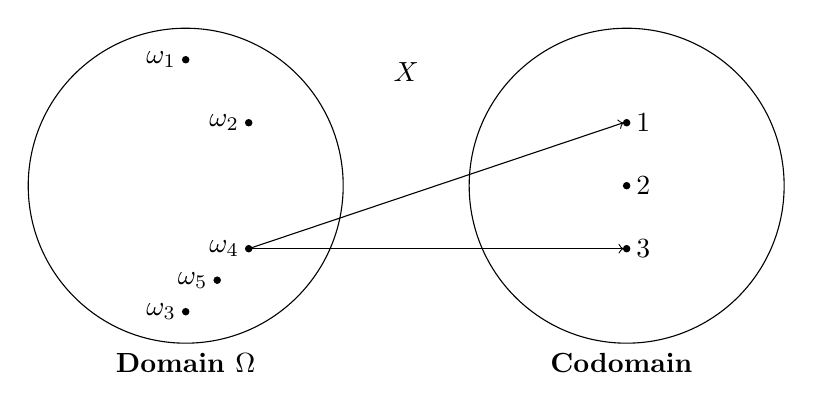
\begin{tikzpicture} [scale = 0.8]
	\draw (0,0) circle (2.5cm) node [below = 2cm] {\textbf{Domain $\Omega$}};
	\draw (7,0) circle (2.5cm) node [below = 2cm] {\textbf{Codomain $\R$}};
	
	\draw [fill = black] (0,2) circle (0.05cm) node [left] {$\omega_1$};
	\draw [fill = black] (1,1) circle (0.05cm) node [left] {$\omega_2$};
	%\draw [fill = black] (0.5,1.5) circle (0.05cm) node [left] {$\omega_3$};
	%\draw [->] (1,1) -- (7-0.05,1);
	%\draw [->] (0,2) -- (7-0.05,1);
	%\draw [->] (0.5,1.5) -- (7-0.05,1);
	\draw [->] (1,-1) -- (7-0.05,1);
	
	\draw [fill = black] (0,-2) circle (0.05cm) node [left] {$\omega_3$};
	\draw [fill = black] (1,-1) circle (0.05cm) node [left] {$\omega_4$};
	\draw [fill = black] (0.5,-1.5) circle (0.05cm) node [left] {$\omega_5$};
	%\draw [->] (0,-2) -- (7-0.05,-1);
	%\draw [->] (0.5,-1.5) -- (7-0.05,-1);
	\draw [->] (1,-1) -- (7-0.05,-1);
	
	\draw [fill = black] (7,1) circle (0.05cm) node [right] {$1$};
	\draw [fill = black] (7,0) circle (0.05cm) node [right] {$2$};
	\draw [fill = black] (7,-1) circle (0.05cm) node [right] {$3$};
	\draw (3.5,1.5) node [above] {$X$};
\end{tikzpicture}
\end{center}
Why is it that this can never happen? \textit{Because it violates the definition of a function.} Functions \textbf{never} map one element from the domain to two different elements in the range (see section \ref{sectionfunctions}). We can never have $X(\omega_4) = 1$ and $X(\omega_4) = 3$ at the same time.

\subsection{Discrete vs continuous random variables} \label{discrete random variable}
\subsubsection{Discrete random variable}
A \textbf{discrete random variable} is a random variable whose outputs are either finite in number, or can be labelled by the natural numbers (i.e., they can be listed somehow). Examples of discrete random variables are:
\begin{itemize}
\item The total shown after rolling two standard dice.
\item The number of heads shown after flipping a fair coin a random number of times.
\item The number of times that it will rain in Wonthaggi next winter.
\end{itemize}

\subsubsection{Continuous random variable} \label{continuous random variable 1}
\noindent A \textbf{continuous random variable} is a random variable whose outputs can only be labelled by the real numbers. We will get onto continuous random variables in more detail in later lectures. For now, some examples of continuous random variables are 
\begin{itemize}
\item The exact blood pressure of patients after taking some drug.
\item The exact height of a randomly selected person.
\item The exact amount of time that it will take you to read this sentence.
\item The exact amount of rainfall in Wonthaggi next winter.
\end{itemize}


\subsection{Example} \label{example8.2}
Suppose we conduct an experiment in which we roll two standard 6 sided dice. Let $Y$ be the descrete random variable that counts the largest out of the two numbers showing. Then
\[
\text{What is} \;\; P(Y < 3)?
\]

\noindent \textit{Solution:} \\
Since $Y$ counts numbers on dice, we know that $1 \leq Y \leq 6$. The set $\set{Y < 3}$ is shorthand for $\set{\omega \in \Omega \mid Y(\omega) < 3}.$ In other words,
\[
\set{Y < 3} =  \set{Y \leq 2} = \set{Y = 1} \cup \set{Y = 2}
\]
We did not include $\set{Y = 3}$ because the inequality ``$<$'' means ``strictly less than 3.''  \\

\noindent Now, we stated in section \ref{disjran} that, since random variables are functions, they must map each outcome to only one number. So, the sets $\set{Y = 1}$ and $\set{Y = 2}$ must not have any outcomes in common; that is, they are disjoint. Hence, using the addition law,
\[
P\brac{\set{Y = 1} \cup \set{Y = 2}} \;\; = \;\; P(\set{Y = 1}) + P(\set{Y = 2}).
\]
Therefore we have
\[
P(Y < 3) \;\; = \;\;  P(Y = 1) + P(Y = 2).
\]
The events themselves are
\begin{align*}
\set{Y = 1} & \;\;=\;\; \set{(1,1)} \\
\set{Y = 2} & \;\;=\;\; \set{(1,2),(2,1),(2,2)}.
\end{align*}
So,
\[
P(Y = 1) = \frac{1}{36}, \qquad \text{and} \qquad P(Y = 2) = \frac{3}{36}.
\]
Therefore
\[
P(Y < 3) \;\; = \;\;  \frac{1}{36} + \frac{3}{36} = \frac{4}{36} = \frac{1}{9}.
\]

\section{Probability mass function} \label{pmf}
The term ``\textbf{probability mass function}'' (abbreviated \textbf{pmf}, and sometimes ``probability frequency function'') is the name that we give to functions like $p(x)$ from example \ref{example8.2}, and from section \ref{sec8.1}, that assign probabilities to particular values or intervals of a random variable. In other words: Let $Z$ be a random variable. Then, for any particular value, or interval, of $Z$, the probability mass function is the function which returns the probability of the associated event. \\

\noindent The probabilities associated with a discrete random variable, say $X$, can be given:
\begin{itemize}
\item As a list; \smallskip
\item In a table;
\item As a rule $\brac{\text{for example, we might specify that }\displaystyle{P(X = x) = \frac{\text{Size of }\set{X=x}}{\text{Size of }\Omega}}};$
\item As a graph (plotting discrete points).
\end{itemize}
As long as $X$ is discrete, then these are all ways to express the probability mass function of~$X$; this is because each of these ways of presenting the probabilities allows us to tell exactly what probability is associated with each value that $X$ can take. \\

\noindent Usually, if we want to indicate that $P(X = x)$ is specified in terms of a rule or a particular function, then we write $p(x)$ to represent the rule, so that \label{symbp(x)}
\[
\boldsymbol{P(X = x) = p(x), \qquad \text{if $p(x)$ is a rule which gives the required probabilities.}}
\]

\subsection{Example} \label{example8.3}
Using the discrete random variable, $Y$, as defined in example \ref{example8.2}, we can create the following table of probabilities. In the table we write both the outcomes $(i,j)$ and $(j,i)$ as just ``$(ij)$'' to save space. This means that if $i \neq j$ then $(ij)$ represents 2 outcomes, rather than just 1.
\begin{center}
\begin{tabular}{c|l|c}
$y$   & Elementary events 		 &$P(Y = y)$ 			\\ \hline
 1	 &(11)		         		 &$\frac{1}{36}$   		\\ 
  2	 &(12),(22)	 	 		 &$\frac{3}{36}$		\\ 
   3	 &(13),(23),(33)	 	 		 &$\frac{5}{36}$		\\ 
    4	 &(14),(24),(34),(44)	 		 &$\frac{7}{36}$		\\ 
     5	 &(15),(25),(35),(45),(55)		 &$\frac{9}{36}$		\\  
      6	 &(16),(26),(36),(46),(56),(66)	 &$\frac{11}{36}$		     
\end{tabular}
\end{center}
Via this table, we have just fully defined the function $P(Y = y)$. We can now refer to the table to find the value of $P(Y = y)$ for any choice of input value. For example,
\[
P(Y = 3) = \frac{5}{36}.
\]
We can also use the table to find the probabilities associated with intervals. Since each of the events $\set{Y = y}$ are disjoint (see section \ref{disjran}) we have, for example (using the addition law)
\[
P(Y \geq 5) \;\; = \;\; P(Y = 5) + P(Y = 6) = \frac{9 + 11}{36} = \frac{20}{36} = \frac{5}{9}. 
\]

\subsection{Example} \label{example8.11}
We can also, if we choose, write the table from example \ref{example8.3} as a list, e.g.,
\[
P(Y = y) = \left\{
  \begin{array}{ll}
    \frac{1}{36},   &\text{if} \; y = 1 \smallskip \\
    \frac{3}{36},   &\text{if} \; y = 2 \smallskip \\
    \frac{5}{36},   &\text{if} \; y = 3 \smallskip \\
    \frac{7}{36},   &\text{if} \; y = 4 \smallskip \\
    \frac{9}{36},   &\text{if} \; y = 5 \smallskip \\
    \frac{11}{36}, &\text{if} \; y = 6 \smallskip \\
  \end{array}
\right.
\]
Or, if we like, we could plot it on a pair of axes:
\begin{center}
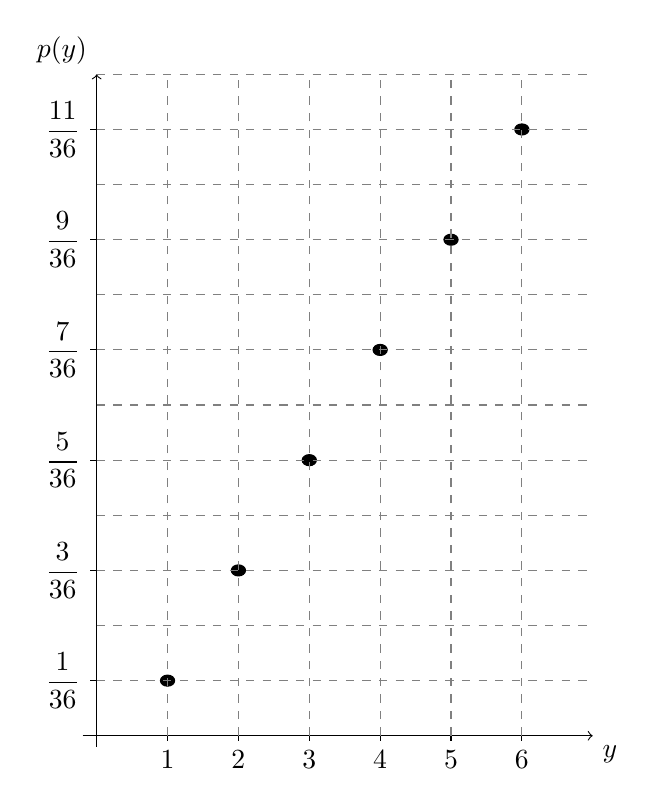
\begin{tikzpicture}[yscale = 0.7,xscale = 0.9]
\draw [->] (-0.2,0) -- (7,0) node [below right] {$y$};
\draw [->] (0,-0.2) -- (0,12) node [above left] {$p(y)$};
\foreach \y in {1,2,3,4,5,6}{
\draw (\y,0.1) -- (\y,-0.1) node [below] {$\y$};
}
\foreach \p in {1,3,5,7,9,11}{
\draw (0.1,\p) -- (-0.1,\p) node [left] {$\displaystyle{\frac{\p}{36}}$};
}
\foreach \y in {1,2,3,4,5,6}{
\draw [fill = black] (\y,2*\y - 1) circle (0.1cm);
}
\foreach \line in {1,2,3,4,5,6}{
\draw [dashed, gray] (\line,0) -- (\line,12);
}
\foreach \line in {1,2,3,4,5,6,7,8,9,10,11,12}{
\draw [dashed, gray] (0,\line) -- (7,\line);
}
\end{tikzpicture}
\end{center}
Or, if we like, we could specify it as a rule, e.g.,
\[
\scases{P(Y = y)}{\displaystyle{\frac{2y-1}{36}}}{y \in \set{1,2,3,4,5,6}}{0}{\text{otherwise}}
\]
To check that this rule is correct, we can plug in each of the possible values of $y$ and check that the rule gives the correct outputs. For example, plugging in $y = 3$: 
\[
P(Y = 3) \;\; = \;\; \frac{2\times3-1}{36} = \frac{5}{36}, \;\; \text{which agrees with our previous definitions of $P(y)$.}
\]

\subsection{Example} \label{example8.12}
Recall the random variable $X$ from example \ref{example8.1} which returns the sum of two standard dice. If we plot the pmf of $X$ we get
\begin{center}
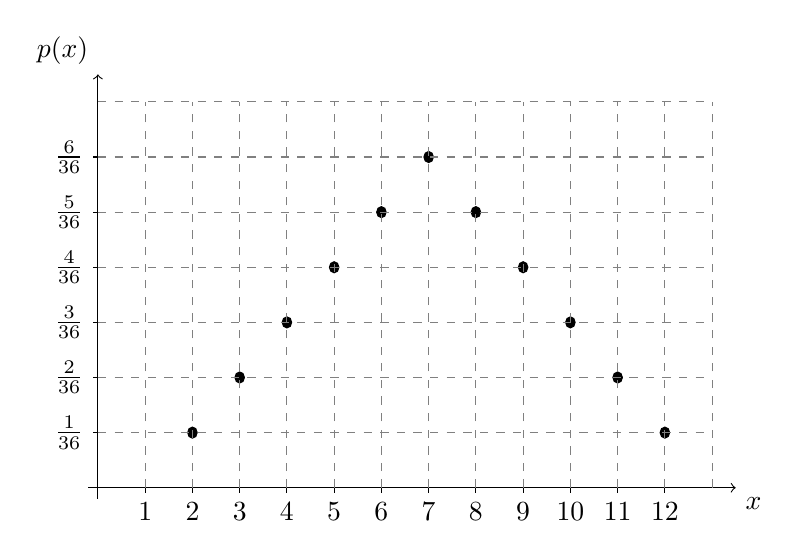
\begin{tikzpicture}[xscale = 0.6,yscale = 0.7]
\def\plength{7}
\def\xlength{13}
\draw [->] (-0.2,0) -- (\xlength + 0.5,0) node [below right] {$x$};
\draw [->] (0,-0.2) -- (0,\plength + 0.5) node [above left] {$p(x)$};
              %axis markings
\foreach \x in {1,2,3,4,5,6,7,8,9,10,11,12}{
\draw (\x,0.1) -- (\x,-0.1) node [below] {$\x$};
}
\foreach \p in {1,2,3,4,5,6}{
\draw (0.1,\p) -- (-0.1,\p) node [left] {$\frac{\p}{36}$};
}
             %plot the points
\foreach \x in {2,3,4,5,6,7}{
\draw [fill = black] (\x,\x-1) circle (0.1cm);
}
\foreach \x in {8,9,10,11,12}{
\draw [fill = black] (\x,13 - \x) circle (0.1cm);
}
	   %add dashed lines
\foreach \line in {1,2,3,4,5,6,7,8,9,10,11,12,13}{
\draw [dashed, gray] (\line,0) -- (\line,\plength);
}
\foreach \line in {1,2,3,4,5,6,7}{
\draw [dashed, gray] (0,\line) -- (\xlength,\line);
}
\end{tikzpicture}
\end{center}
As you can see, the graphs of different probability mass functions will have distinct shapes. As we increase the amount of data, the shape usually becomes more apparent. These shapes tend to fall naturally into families of shapes; that is, we can group pmfs together based on properties that their shapes have in common. The goal of modelling data is to find the best ``shape'' to fit to our data, so that we can capture the features of our data and extrapolate to make predictions; we can then study whichever mathematical model that we have chosen. 

\section{Cumulative distribution function} \label{cdf}
A \textbf{cumulative distribution function} (abbreviated \textbf{cdf}) is always denoted by capital letter $F.$ The cdf is defined so that, for any random variable, $X$, \label{symbF(x)}

  	\bigskip
	
	\hfil\fbox{
	\begin{minipage}{0.3\columnwidth}{
	
	\vskip 0.02cm
	\begin{center}
	$F(x) = P(X \leq x), \;\;\;$ \text{where $x \in \R$.}
	\end{center}
	}
	\end{minipage}}
	\bigskip
	\bigskip

\noindent Let $a$ be a real number, then, for a discrete random variable, $F(a)$ is the sum of the probabilities of all values of the random variable up to and including the value $a$. This is exaclty what we did in example \ref{example8.2}, when we found $P(Y < 3)$, which was equivalent to $P(Y \leq 2)$. In other words, we found $F(2)$ in that example. \\

\noindent For any two real numbers $a$ and $b$, we can use the cdf to express $P(a < X \leq b)$. We have,
\begin{align*}
P(a < X \leq b) & = P(X \leq b) - P(X \leq a) \\
		       & = F(b) - F(a).
\end{align*}
So we have

  	\bigskip
	
	\hfil\fbox{
	\begin{minipage}{0.4\columnwidth}{
	
	\vskip 0.02cm
	\begin{center}
	$P(a < X \leq b) = F(b) - F(a)$
	\end{center}
	}
	\end{minipage}}
	\bigskip
	\bigskip
%newbox



  	\bigskip
	
	\hfil\fbox{
	\begin{minipage}{1\columnwidth}{
	
	\vskip 0.02cm
	\begin{center}
\noindent Perhaps the best way to think of this intutively is to compare it to the following way of expressing the interval $(a,b]$ on a real number line:
\begin{center}
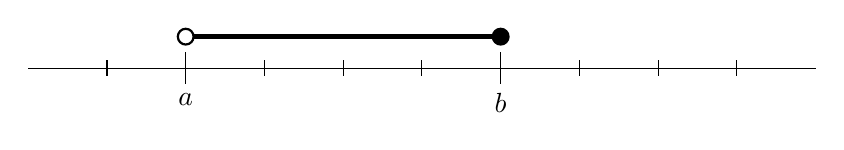
\begin{tikzpicture}
\draw (0,0) -- (10,0);
\draw (2,0.2) -- (2,-0.2) node [below] {$a$};
\draw (6,0.2) -- (6,-0.2) node [below] {$b$};
\foreach \x in {1,3,4,5,7,8,9}{
\draw (\x,0.1) -- (\x,-0.1);
}
\draw [thick] (2,0.4) circle (0.1cm);
\draw [thick, fill = black] (6,0.4) circle (0.1cm);
\draw [ultra thick] (2.1,0.4) -- (6,0.4);
\end{tikzpicture}
\end{center}

The white circle above $a$ indicates that we want to exclude the point $a$ from the interval, and the black circle above $b$ indicates that we want to include the point $b$ in the interval. We can obtain $(a,b]$ by taking the interval $(-\infty,b]$:
\begin{center}
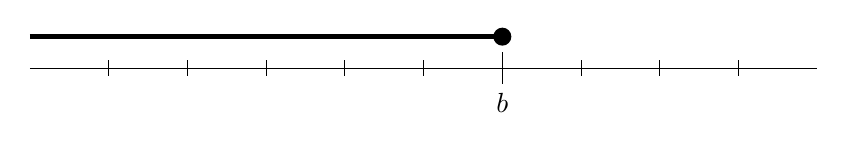
\begin{tikzpicture}
\draw (0,0) -- (10,0);
%\draw (2,0.2) -- (2,-0.2) node [below] {$a$};
\draw (6,0.2) -- (6,-0.2) node [below] {$b$};
\foreach \x in {1,2,3,4,5,7,8,9}{
\draw (\x,0.1) -- (\x,-0.1);
}
%\draw [thick] (2,0.4) circle (0.1cm);
\draw [thick, fill = black] (6,0.4) circle (0.1cm);
\draw [ultra thick] (0,0.4) -- (6,0.4);
\end{tikzpicture}
\end{center}
and subtracting (or excluding) the interval $(-\infty,a]$:
\begin{center}
\begin{tikzpicture}
\draw (0,0) -- (10,0);
\draw (2,0.2) -- (2,-0.2) node [below] {$a$};
%\draw (6,0.2) -- (6,-0.2) node [below] {$b$};
\foreach \x in {1,3,4,5,6,7,8,9}{
\draw (\x,0.1) -- (\x,-0.1);
}
%\draw [thick] (2,0.4) circle (0.1cm);
\draw [thick, fill = black] (2,0.4) circle (0.1cm);
\draw [ultra thick] (0,0.4) -- (2,0.4);
\end{tikzpicture}
\end{center}
This leaves us with the interval $(a,b]$, as required. So, if we let the ``-'' symbol represent the exclusion of one set from another, then $\set{x \mid a < x \leq b} = \set{x \mid x \leq b} - \set{x \mid x \leq a}$.
	\end{center}
	}
	\end{minipage}}
	\bigskip
	\bigskip


\noindent If $X$ is a discrete random variable, then the plot of $F$ will have ``steps'' in it. For example, let's plot $F$ for the random variable $Y$ from example \ref{example8.2}. We will need the following calculations:
\begin{align*}
F(1) & = P(Y \leq 1) = P(Y = 1) = \frac{1}{36} \\
F(2) & = P(Y \leq 2) = P(Y = 1) + P(Y = 2) = \frac{1}{36} + \frac{3}{36} = \frac{4}{36} \\
F(3) & = \ldots + P(Y = 3) = \frac{4}{36} + \frac{5}{36} = \frac{9}{36} \\
F(4) & = \ldots + P(Y = 4) = \frac{9}{36} + \frac{7}{36} = \frac{16}{36} \\
F(5) & = \ldots + P(Y = 5) = \frac{16}{36} + \frac{9}{36} = \frac{25}{36} \\
F(6) & = \ldots + P(Y = 6) = \frac{25}{36} + \frac{11}{36} = \frac{36}{36}. 
\end{align*}
Now, using this information to plot $y$ versus $F(y)$, we get:
\begin{center}
\begin{tikzpicture}[yscale = 0.3,xscale = 0.9]
\draw [->] (-0.2,0) -- (7,0) node [below right] {$y$};
\draw [->] (0,-0.2) -- (0,37) node [above left] {$F(y)$};
\foreach \y in {1,2,3,4,5,6}{
\draw (\y,0.5) -- (\y,-0.5) node [below] {$\y$};
}
\foreach \p in {1,4,9,16,25,36}{
\draw (0.1,\p) -- (-0.1,\p) node [left] {$\frac{\p}{36}$};
}
%\foreach \y in {1,2,3,4,5,6}{
%\draw [fill = black] (\y,2*\y - 1) ellipse (0.1cm and 0.3cm);
%}
\draw [ultra thick] (-0.2,0) -- (1-0.1,0);
\draw [fill = white] (1,0) ellipse (0.1cm and 0.3cm);
\draw [fill = black] (1,1) ellipse (0.1cm and 0.3cm);

\draw [ultra thick] (1,1) -- (2,1);
\draw [fill = white] (2,1) ellipse (0.1cm and 0.3cm);
\draw [fill = black] (2,4) ellipse (0.1cm and 0.3cm);

\draw [ultra thick] (2,4) -- (3,4);
\draw [fill = white] (3,4) ellipse (0.1cm and 0.3cm);
\draw [fill = black] (3,9) ellipse (0.1cm and 0.3cm);

\draw [ultra thick] (3,9) -- (4,9);
\draw [fill = white] (4,9) ellipse (0.1cm and 0.3cm);
\draw [fill = black] (4,16) ellipse (0.1cm and 0.3cm);

\draw [ultra thick] (4,16) -- (5,16);
\draw [fill = white] (5,16) ellipse (0.1cm and 0.3cm);
\draw [fill = black] (5,25) ellipse (0.1cm and 0.3cm);

\draw [ultra thick] (5,25) -- (6,25);
\draw [fill = white] (6,25) ellipse (0.1cm and 0.3cm);
\draw [fill = black] (6,36) ellipse (0.1cm and 0.3cm);

\draw [dashed, gray] (1,0+0.3) -- (1,1);
\draw [dashed, gray] (2,1+0.3) -- (2,4);
\draw [dashed, gray] (3,4+0.3) -- (3,9);
\draw [dashed, gray] (4,9+0.3) -- (4,16);
\draw [dashed, gray] (5,16+0.3) -- (5,25);
\draw [dashed, gray] (6,25+0.3) -- (6,36);
%\foreach \line in {1,2,3,4,5,6}{
%\draw [dashed, gray] (\line,0) -- (\line,12);
%}
%\foreach \line in {1,2,3,4,5,6,7,8,9,10,11,12}{
%\draw [dashed, gray] (0,\line) -- (7,\line);
%}
\end{tikzpicture}
\end{center}
Notice that $F(6) = 1$. This is because $6$ is the maximum element in the domain of $F$; in other words, 
\[
\set{Y \leq 6} = \set{Y = 1} \cup \set{Y = 2} \cup \set{Y = 3} \cup \set{Y = 4} \cup \set{Y = 5} \cup \set{Y = 6} \;\; = \;\; \Omega,
\]
and we know from probability measure axiom 1 that $P(\Omega) = 1$, so of course $F(6) = 1$. \\

\noindent \textbf{In general, if $X$ is a discrete random variable, then the sum of all of the individual probabilities of the values that $X$ can take must always be equal to 1.} In other words, if we say that $X$ can take values from the set $\set{x_1,x_2,x_3,\ldots}$, then

  	\bigskip
	
	\hfil\fbox{
	\begin{minipage}{0.45\columnwidth}{
	
	\vskip 0.02cm
	\begin{center}
	$\displaystyle{\sum_{x_i}P(X = x_i) \; = \; \sum_{x_i}p(x_i) = 1.}$
	\end{center}
	}
	\end{minipage}}
	\bigskip
	\bigskip
	
\noindent This is clearly a consequence of probability measure axiom 1, because taking the sum of probabilities of every possible value of $X$ is equivalent to finding the probability of~$\Omega$. \\

\noindent The following properties are always satisfied by cumulative distribution functions:
\begin{itemize}
\item As $x \rightarrow \infty, \;\;\; F(x) \rightarrow 1;$
\item As $x \rightarrow -\infty, \;\;\; F(x) \rightarrow 0;$
\item A cumulative distribution function is always non-decreasing (they either increase or remain the same).
\end{itemize}
The first dot point follows, as we have already observed, from probability measure axiom 1. The second second dot point is related to a consequence of the probability measure axioms (that $P(\varnothing) = 0$). The final dot point is easy to prove: For any real numbers, $a$ and $b$, if $b \geq a$ then
\begin{align*}
F(b) & = P(X \leq b) \\
	& = P(\set{X \leq a} \cup \set{a < X \leq b}) \\
	& = P(X \leq a) + P(a < X \leq b) \\
	& \geq P(X \leq a) \tag{since $P(a < X \leq b) \geq 0$} \\
	& = F(a).
\end{align*}
Hence $F(b) \geq F(a)$ whenever $b \geq a$; that is, F is always non-decreasing.

\section{Independence and discrete random variables} \label{indep(discreterand)}
In lecture \ref{independence}, we already covered the definitions of pairwise and mutual independence for events; but \textbf{when should we say that two \textit{discrete random variables}, $X$ and $Y$, are independent?} \\

\noindent Since $X$ and $Y$ can each possibly take many different values, it makes sense that a sensible definition of independence would require that \textit{every} event, specified by every possible value of $X$ should be independent from \textit{every} event, specified by every possible value value of $Y$. \\

\noindent In other words, for every output, $x$, of $X$, and for every output, $y$, of $Y$, we want
\[
\set{X = x} \;\; \text{to be independent from} \;\; \set{Y = y}.
\]
Recalling our definition of independence from lecture \ref{independence}, this means that we require
\[
P\brac{\set{X = x} \cap \set{Y = y}} = P\brac{X = x}P\brac{Y = y}.
\]
Put more accurately, if the outputs of $X$ belong to the set $\set{x_1, x_2, x_3, \ldots}$ and the outputs of $Y$ belong to the set $\set{y_1, y_2, y_3, \ldots}$, then $X$ and $Y$ are independent if, for all possible $i,j$:

  	\bigskip
	
	\hfil\fbox{
	\begin{minipage}{0.6\columnwidth}{
	
	\vskip 0.02cm
	\begin{center}
	$P(X = x_i \;\; \textit{and} \;\; Y = y_j) = P(X = x_i)P(Y = y_j)$
	\end{center}
	}
	\end{minipage}}
	\bigskip
	\bigskip
	
\noindent Where we have used the word ``\textit{and}'' because, in this context, it is equivalent to ``$\cap$.'' 

\subsection{Example}
Consider the discrete random variable, $X$, from example \ref{example8.1}, and the discrete random variable, $Y$, from example \ref{example8.2}. These two variables are \textit{not} independent. In order to prove this, we \textbf{only need to find one pair of values, $\boldsymbol{x}$ and $\boldsymbol{y},$} for which
\[
P(X = x \;\; \textit{and} \;\; Y = y) \neq P(X = x)P(Y = y).
\] 
In section \ref{sec8.1} we found that $P(X = 4) = \frac{1}{12}$, and in example $\ref{example8.2}$ we found that $P(Y = 2) = \frac{3}{36} = \frac{1}{12}$. So taking $x = 4$, and taking $y = 2$, the right hand side of the above expression becomes
\[
 P(X = x)P(Y = y) = \frac{1}{12}\times\frac{1}{12} = \frac{1}{24}.
\]
To find the left hand side we need to find the event
\[
X = 4 \;\; \textit{and} \;\; Y = 2.
\]
Which, written more formally, is the event
\[
\set{X = 4} \cap \set{Y = 2}.
\]
Written even more formally, this is the event
\[
\set{\omega \in \Omega \mid X(\omega) = 4} \cap \set{\omega \in \Omega \mid Y(\omega) = 2}.
\]
Going back to a complete lack of formality, we can rewrite this as
\[
\set{\text{The sum of the two dice is 4}} \;\; \textit{and} \;\; \set{\text{The largest number on the two dice is 2}}.
\]
Now, with a little thought, we can see that this is only true when we roll $(2,2).$ Hence,
\[
P(X = 4 \;\; \textit{and} \;\; Y = 2) = P((2,2)) = \frac{1}{36}.
\]
In conclusion,
\[
P(X = 4 \;\; \textit{and} \;\; Y = 2) = \frac{1}{36} \neq \frac{1}{24} =  P(X = x)P(Y = y).
\]
So, since we have shown that there is at least one pair of values, $x = 4$ and $y = 2$, such that the events specified by the random variables $X$ and $Y$ are not independent, we conclude that $X$ and $Y$ are not independent.


%THIS COULD REALLY USE AN EXAMPLE WHERE THE EVENTS ARE INDEPENDENT.